\section{Ejercicio 1 - Creacion de un proyecto de Analisys Services}  

Antes de comenzar este ejercicio debera crear:

Una carpeta en el escritorio con el nombre: Proyecto2CuboCarnet

1. Crear un nuevo Proyecto en Visual Studio 2019 , Hacer clic en Business Intelligence.

	\begin{center}
	
\includegraphics[width=\columnwidth]{images/task1/img1}
	\end{center}	


2. Seleccione el tipo de Proyecto multidimensional y de minería de datos de Analysis Services
	\begin{center}
	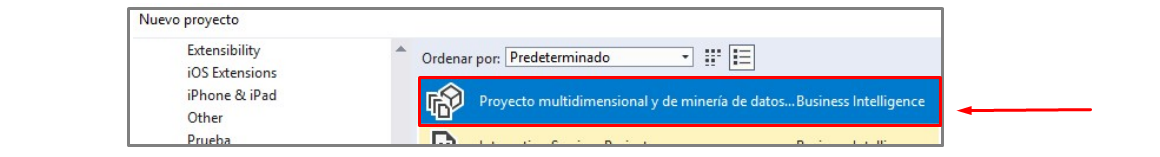
\includegraphics[width=\columnwidth]{images/task1/img2}
	\end{center}	

3. Colocar como nombre de proyecto: CuboAdventureWorks2012
		
4. Seleccionar la carpeta creada en el escritorio

	\begin{center}
	
\includegraphics[width=\columnwidth]{images/task1/img4}
    \end{center}	

5. . Hacer clic en Aceptar

    